\chapter{Digitalisierte Dokumente}
\label{chap:documents}
% Warum scannt man Dokumente

% Was für Dokumente werden gescannt

% 
Menschen erstellen Dokumente schon seit mehr als 4000 Jahren \parencite[13]{SmithDocumentCreationImage2014}. Dokumente, von Tontafeln (siehe \cref{fig:tablet})
bis hinzu rein digitalen Dokumenten, ermöglichen Kommunikation über zeitliche und ortliche Grenzen hinweg. 
Diese Technologie ist aus unserer modernen Kultur nicht mehr wegzudenken.  
Seit den 50er Jahren begann die Forschung im Bereich der Optischen Zeichenerkennung 
(engl. OCR)\autocite{DoermannHandbookdocumentimage2014}. OCR fand zuerst Einsatz in genau 
spezifizierten Problembereichen zum Beispiel die Erkennung von Druckbuchstaben einer Schreibmaschine. 
Je mehr Dokumente digitalisiert wurden, desto klarer wurde es das Dokumente mehr als 
eine Kette von Zeichen sind. 
Information können in Dokumenten über die Position der Zeichen und Skalierung von Zeichen vermittelt werden.
Zum anderen bestehen Dokumente aus Inhalten die semantische Bedeutung haben, aber nicht als Zeichenkette codiert werden können. 
%Eine Randnotiz
%\marginnote{Der Bezug dieses Satzes zum Text wird durch die Position verdeutlicht} setzt sich durch Formatierung und Position vom restlichen Text ab. 
\begin{marginfigure}
    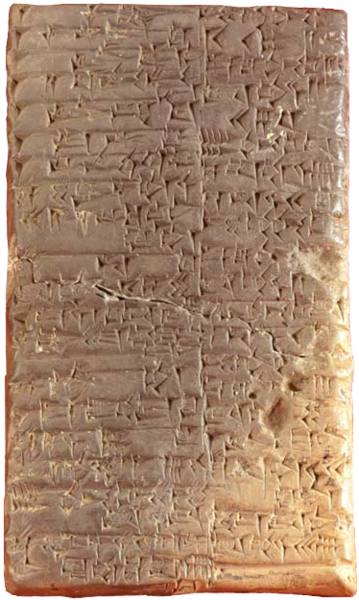
\includegraphics[width=\textwidth]{figures/img/359px-Cuneiform_script2.png}
    \caption{Königsliste (2047 Jahre v.Chr. \cite{DavidgeCuneiformscript2jpg})}
    \label{fig:tablet}
\end{marginfigure}


Wirtschaftsinteressen trieben die Entwicklungen von Dokumentenverarbeitungssystemen in einigen Bereichen sehr weit voran, wie 
zum Beipspiel bei der Verarbeitung von Geschäftsbriefen und Formularauswertung.
Eine Spezialisierung auf bestimmte Dokumentenklassen ist immer noch eine notwendigkeit angesichts der unzähligen, veränderbaren und nicht fest gelegten Gestaltungsmöglichkeiten für Dokumente \parencite[69]{BairdEvolutionDocumentImage2014}.

\section{Dokumente}
Typischerweise beschreiben wir ein Dokument als ein Papier mit einer Nachricht darauf. Diese Nachricht kann textueller Art sein, dass beudeutet Glyphen die in horizontalen oder vertikalen Lininen angeordnet sind (je nach Sprache)\parencite{BairdBriefHistoryDocuments2014}. Diese Textlininen sind dann meist in Textblöcken organisiert. Dokumente können auch grafische Inhalte haben. 
\qq{Warum sind alte Dokumente sind noch schwerer?}
Dokumente die mit modernen maschinellen Verfahren hergestellt sind einheitlicher in der Hinsicht, dass sie nicht nur einen einheitlichen Schriftsatz besitzen sondern auch alle anderen typografischen Parameter sind einheitlicher, auch Textlinien sind gerade und parallel.  

\section{Digitale Bibliotheken}
\qq{Was ist eine digitale Bibliothek?}
Immer mehr Bibliotheken und Archive arbeiten daran Sammlungen von Dokumenten zu digitalisieren und im Internet zur Verfügung zu stellen. 
Digitale Sammlungen sind dann nicht mehr an die Restriktionen von analogen Dokumenten gebunden und können deshalb auch seltene Dokumente oder Einzelstücke einer großen Menge von Nutzern züganglich machen.
Dies erleichtert besonders die Forschung an  historischen Dokumenten, da diese oft so wertvoll und fragil sind, dass die Lagerung und Nutzung der Originale strengen Auflagen unterliegen.

Die Digitalisierung ist aber nicht kostenfrei. Die Kosten belaufen sich bei Digitalisierungsprojekten in Deutschland auf etwa 10 bis 50 Cent pro Seite \parencite{OpitzWorkshopMassendigitalisierungsprojekteDeutschen2009}.
Die komplete Erfassung kann nochmals teurer sein, da die Erfassung von Strukturdaten zusätzliche Kosten verursacht. 
Im Digitalisierungsprojekt \emph{dünnhaupt digital} ist die Strukturdatenerfassung mit 40 Cent pro Seite der größte Ausgabenpunkt.
\cite{OpitzWorkshopMassendigitalisierungsprojekteDeutschen2009} bemerkt auch, dass die Volltextgenerierung mittels OCR nicht für eine sinnvolle Onlinenutzung nicht ausreichend ist. Erst die Erfassung von Seitenstrukturen erlaubt  ``einen gezielten Zugriff auf  logische Texteinheinten'' \parencite[372]{OpitzWorkshopMassendigitalisierungsprojekteDeutschen2009}.

\qq{Anforderungen an digitale Dokumente?}
Gescannnte Dokumente ohne eine symbolische Kodierung laufen Gefahr irrelevant zu werden,
da ihre Handhabung viel schlechter ist als die von ``purely digital information'' \parencite[10]{BairdDigitallibrariesdocument2003}.
 
\section{Datenrepresentation}

Nichtdestotrotz sind enorm viele digitalisierte Dokumente im Internet verfügbar.
Die größten Sammlungen sind unteranderem Google Books und das Internet Archive.
Diese Sammlungen haben das Ziel möglichst viele Dokumente bereitzustellen. 
Die Qualität kann dabei stark variieren.

Andere Sammlungen beschränken sich auf einen klarer definierten Korpus und Digitalisierungsmethoden.

Die digitalisierte Sammlungen der Staatsbibliothek zu Berlin \cite{StaatsbibliothekzuBerlinDigitalisierteSammlungenStaatsbibliothek2016} umfasst \research{?? Dokumente}.

\research{Bach digital}


\qq{Vereinheitlichung}
International Image Interoperability Framework \cite{IIIFInternationalImageInteroperability2018}


\section{Schritte in der Verarbeitung von Dokumentenbildern}
Die Dokumentensegmetierung ist ein Vorverarbeitungsschritt für weitere Schritte der Dokumentenverarbeitung.
